\subsection{Flow rate in a tube}
	\begin{figure}[H]
		\centering
		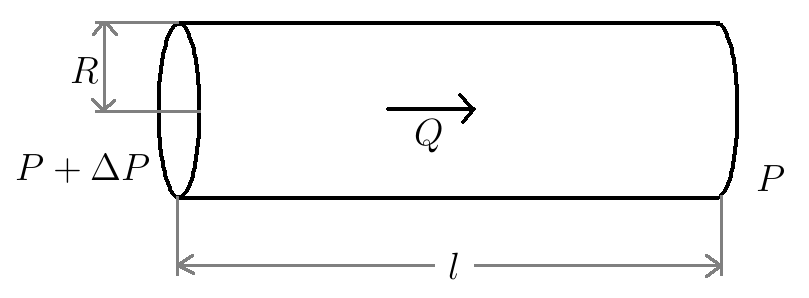
\includegraphics[width=0.7\textwidth]{fig_flow-rate-pousielle-article}
		\caption{Tube with pressure difference across its ends causing fluid to flow.}
		\label{fig_shape-meniscus}
	\end{figure}
	The flow rate of a viscous fluid through a thin tube is given by the Hagen–Poiseuille equation:
	
	\begin{equation} \label{eq:flow-rate}
		Q = \frac{\pi}{8\mu} \frac{\Delta P}{l} R^4
	\end{equation}
	
	Here, $Q$ is the volumetric flow rate in $[m^3/s]$, $\Delta P$ is the pressure difference between the ends of the tube, $\mu$ is the viscosity in $[kg/m.s]$, $l$ is the length of the tube, $R$ is the radius of the tube.
	
\subsection{Flow rate in a tube with one meniscus}
	\begin{figure}[H]
		\centering
		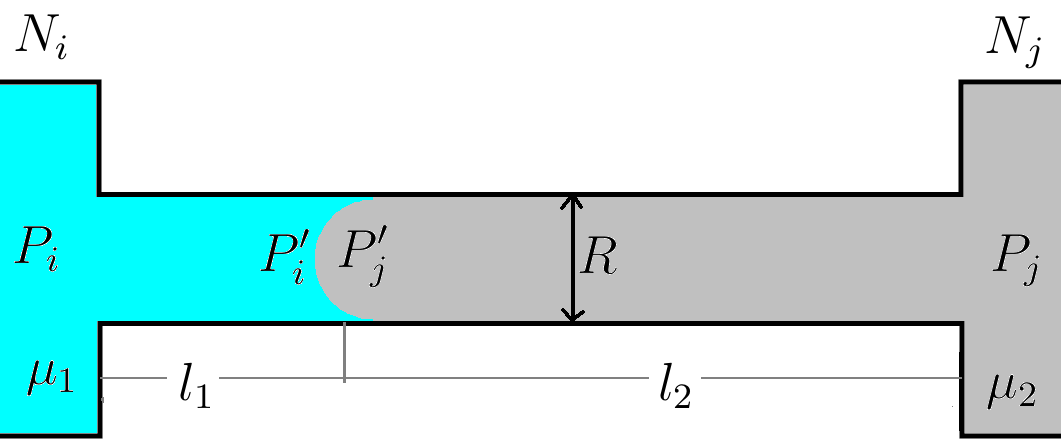
\includegraphics[width=0.6\textwidth]{fig_capillary_pressure_in_tube_1mns_blue}
		\caption{Orientation of the meniscus, the convex side contains wetting fluid while the concave side contains non-wetting fluid.}
		\label{fig_capillary_pressure_in_tube_1mns_blue}
	\end{figure}
	
	In figure \ref{fig_capillary_pressure_in_tube_1mns_blue}, node $N_{i}$ kept at a pressure of $P_{i}$, and is filled with a wetting fluid of viscosity $\mu_{1}$. Node $N_{j}$ kept at a pressure of $P_{j}$ is filled with a non-wetting fluid of viscosity $\mu_{2}$.
	
	Since in figure \ref{fig_capact-of-water} the wetting fluid rises against gravity, the pressure on the convex side of the meniscus is lower than on the concave side:
	
	\begin{equation}
		P_{i}' < P_{j}'
	\end{equation}
	
	The pressure jump is given by:
	
	\begin{equation} \label{eq:capillary_pressure_mns}
		P_{j}' - P_{i}' = \frac{2 \sigma}{R}
	\end{equation}
	
	Here, $\sigma$ is the coefficient of surface tension in $[Pa.m]$ or $[kg/s]$.
	
	In figure \ref{fig_capillary_pressure_in_tube_1mns_blue}, when $P_{i} = P_{j}$, the fluids will flow from $N_{i}$ to $N_{j}$ due to the capillary pressure. Therefore, when $P_{i} > P_{j}$, the fluids will also move from $N_{i}$ to $N_{j}$.
		
	Separating figure \ref{fig_capillary_pressure_in_tube_1mns_blue} into two tubes of lengths $l_{1}$ and $l_{2}$, containing fluids of viscosity ${\mu}_1$ and ${\mu}_2$. The flow rates of the tubes, from equation \ref{eq:flow-rate} are given by:
	
	\begin{equation} \label{eq:flow-rate-first}
		Q_i = \frac{\pi}{8{\mu}_1} \frac{P_i - P^{'}_i}{l_1} R^4
	\end{equation}
	
	\begin{equation} \label{eq:flow-rate-second}
		Q_j = \frac{\pi}{8{\mu}_2} \frac{P^{'}_j - P_j}{l_2} R^4
	\end{equation}
	
	The fluids are not compressible, then:
	\begin{equation} \label{eq:flow-rate-volume-same}
		Q_i = Q_j = Q
	\end{equation}
	
	Using equation \ref{eq:flow-rate-volume-same}, and multiplying equations \ref{eq:flow-rate-first} and \ref{eq:flow-rate-second} by ${\mu}_1 l_1$ and ${\mu}_2 l_2$ respectively:
	
	\begin{equation} \label{eq:flow-rate-first-coeff}
		Q \mu_{1} l_1 = \frac{\pi}{8} (P_i - P^{'}_i) R^4
	\end{equation}
	
	\begin{equation} \label{eq:flow-rate-second-coeff}
		Q \mu_{2} l_2 = \frac{\pi}{8} (P^{'}_j - P_j) R^4
	\end{equation}

	Adding equation \ref{eq:flow-rate-first-coeff} and \ref{eq:flow-rate-second-coeff}:
	
	\begin{equation} \label{eq:flow-rate-intermediate}
		Q({\mu}_1 l_1 + {\mu}_2 l_2) = \frac{\pi}{8}R^4(P_i - P_j + P^{'}_j - P^{'}_i)
	\end{equation}
	
	Let, the pressure difference between the nodes be defined as:
	\begin{equation} \label{eq:def-pressure-difference} 
		\Delta P_{ij} = P_{i} - P_{j}
	\end{equation}
	
	Substituting \ref{eq:def-pressure-difference} and \ref{eq:capillary_pressure_mns} into equation \ref{eq:flow-rate-intermediate}, and after rearranging:
	
	\begin{equation} \label{eq:flow-rate-1mns-basic}
		Q = \frac{\pi R^4}{8({\mu}_1 l_1 + {\mu}_2 l_2)} \left( \Delta P_{ij} + \frac{2\sigma}{R} \right)
	\end{equation}
	
	Defining $M$ as the viscosity parameter:
	\begin{equation}
		M = \sum_{k} \mu_{k} \frac{l_{k}}{l}
	\end{equation}
	
	Equation \ref{eq:flow-rate-1mns-basic} becomes:
	\begin{equation} \label{eq:flow-rate-1mns-basic-m}
		Q = \frac{\pi R^4}{8Ml} \left( \Delta P_{ij} + \frac{2\sigma}{R} \right)
	\end{equation}
	
\subsection{Flow rate in a tube with multiple meniscus}
	
	\begin{figure}[H]
		\centering
		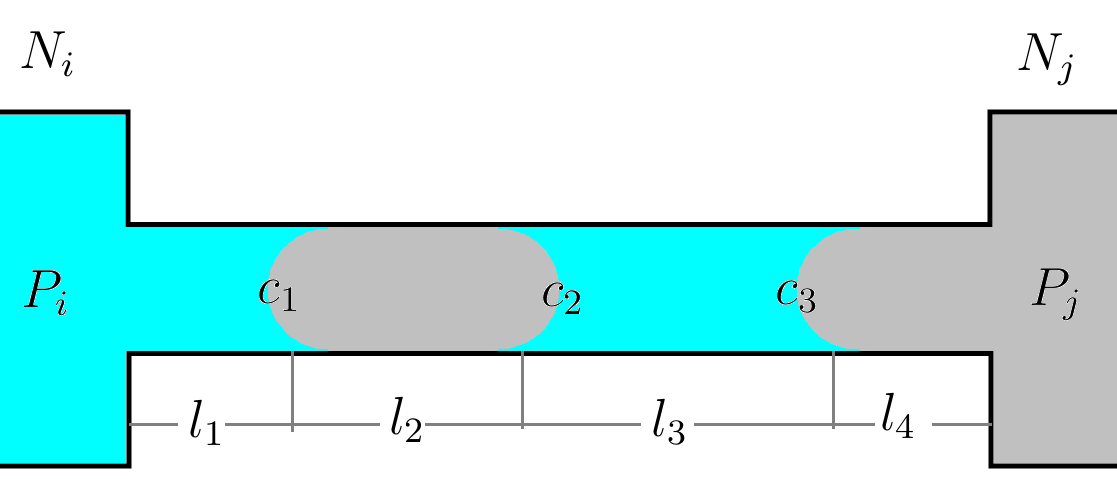
\includegraphics[width=0.6\textwidth]{fig_capillary_pressure_in_tube_3mns}
		\caption{Capillary pressure contribution, $s = 1$}
		\label{fig:capillary_pressure_in_tube_3mns}
	\end{figure}
	
	Let the capillary pressures be denoted by the following:
	\begin{equation}
		c_1 = -c_2 = c_3 = \frac{2 \sigma}{R}
	\end{equation}
	
	Then for figure \ref{fig:capillary_pressure_in_tube_3mns}, the flow rate is given by:
	
	\begin{equation}
		Q = \frac{\pi R^4}{8Ml} \left( \Delta P_{ij} + c_1 + c_2 + c_3 \right)
	\end{equation}
	
	\begin{equation}
		Q = \frac{\pi R^4}{8Ml} \left( \Delta P_{ij} + \sum_{k} c_{k} \right)
	\end{equation}
	
	Flow rate for an arbitrary number of meniscus for a cylindrical tube, is given by:
	
	\begin{equation}
		Q = \frac{\pi R^4}{8Ml} \left( \Delta P_{ij} + \frac{2s \sigma}{R} \right)
	\end{equation}
	
	Here $s$ is defined as a function of orientation of the meniscus or the direction the convex side of the meniscus points $d$ and the number of meniscus $n_{mns}$:
	
	\begin{equation} \label{eq:sign-func-def}
		s(d, n_{mns}) = 
		\begin{dcases}
			-1,&\text{$n_{mns}$ = 1, convex side points away from $N_{i}$}\\
			0,&\text{$n_{mns}$ = 0, 2}\\
			+1,&\text{$n_{mns}$ = 1, convex side points towards $N_{i}$}
		\end{dcases}
	\end{equation}
	
	In our model, the data structure does not accommodate more than 2 meniscus in a tube, therefore we limit the definition of $s$ to a maximum of 2. $s$ for various other configurations:
	
	\begin{figure}[H]
		\centering
		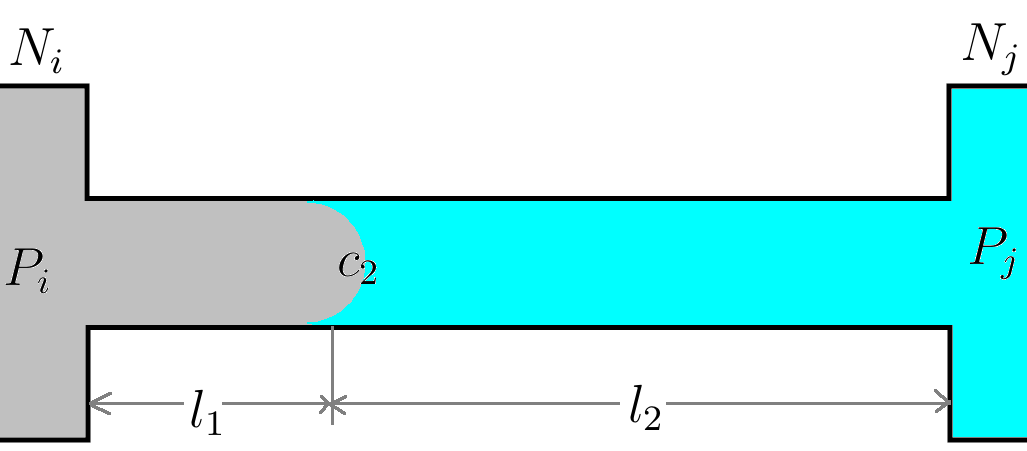
\includegraphics[width=0.6\textwidth]{fig_capillary_pressure_in_tube_1mns_grey}
		\caption{Capillary pressure contribution, $s = -1$}
		\label{fig:capillary_pressure_in_tube_1mns_grey}
	\end{figure}
	
	\begin{figure}[H]
		\centering
		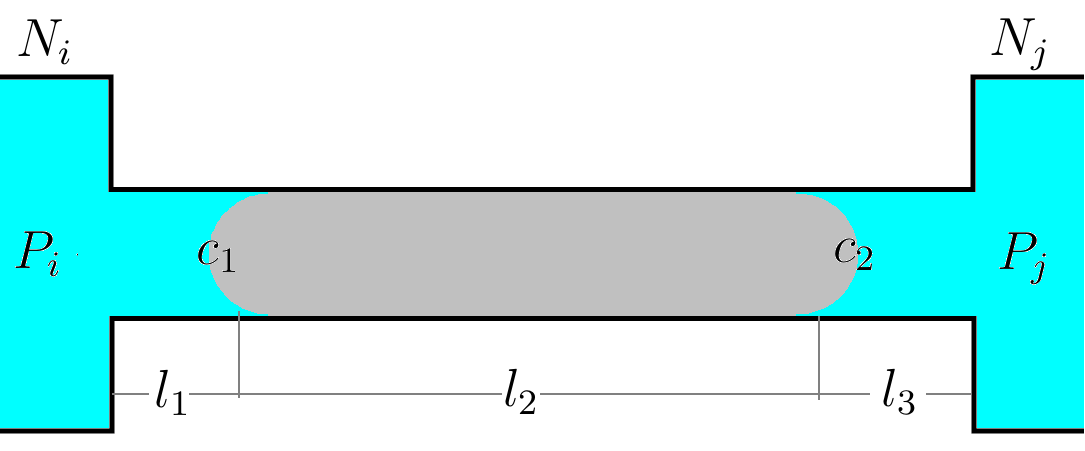
\includegraphics[width=0.6\textwidth]{fig_capillary_pressure_in_tube_2mns}
		\caption{Capillary pressure contribution, $s = 0$}
		\label{fig:capillary_pressure_in_tube_2mns}
	\end{figure}
	
\subsection{Set of linear equations for a node} \label{sec:linear-equ}
	\begin{figure}[H]
		\centering
		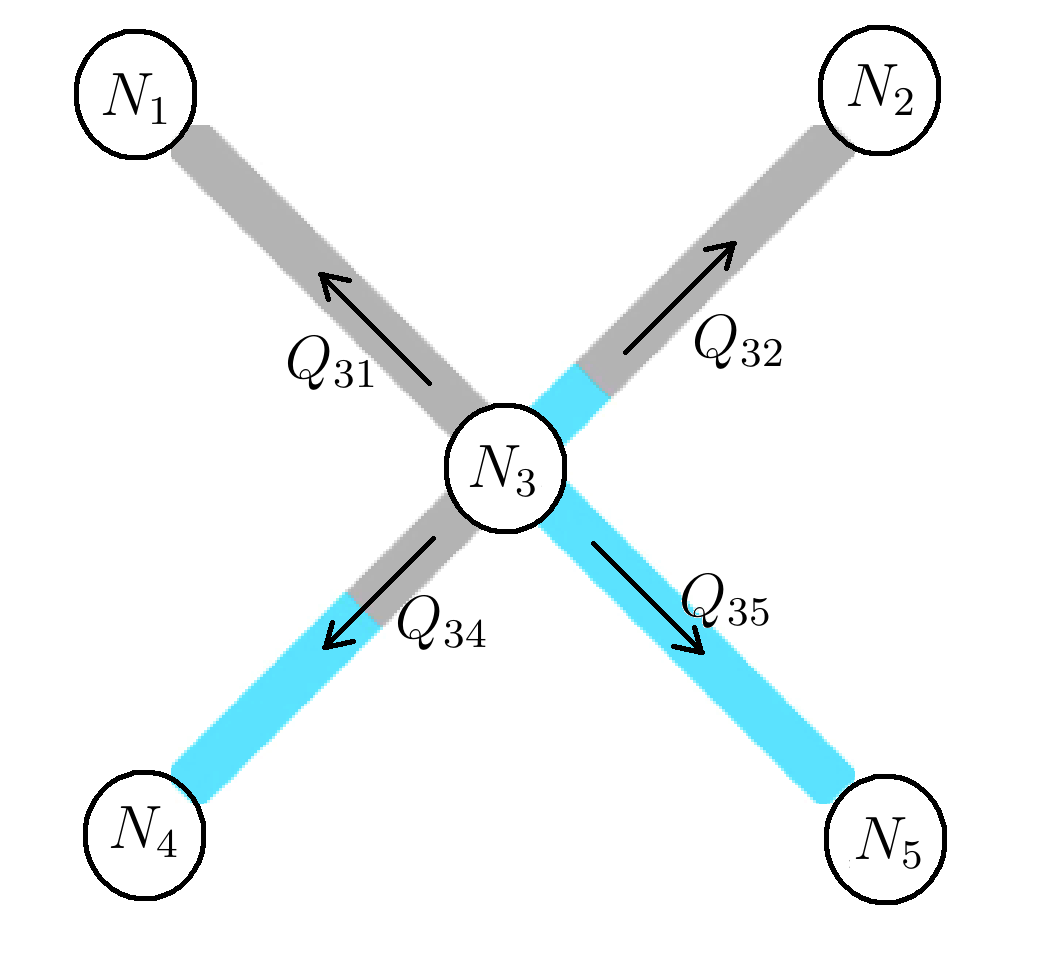
\includegraphics[height=8cm]{fig_simple-5-nodes}
		\caption{Capillary pressure contribution, $s = 0$}
		\label{fig:simple-5-nodes}
	\end{figure}
	
	Let us apply our method on a simple system consisting of only 5 nodes.
	Note that all $Q$ point outward. It is only to denote the direction. In order to preserve the law of conservation of volume, the $Q$'s will have different signs.

	

	Since there are 4 tubes, we can write 4 equations according to \ref{eq:flow-rate-main}
	
	\[ Q_{31} = \frac{\pi R_{31}^4}{8lM_{31}}(R_{31}\Delta P_{31} + 2s_{31}\sigma) \]
	\[ Q_{32} = \frac{\pi R_{32}^4}{8lM_{32}}(R_{32}\Delta P_{32} + 2s_{32}\sigma) \]
	\[ Q_{34} = \frac{\pi R_{34}^4}{8lM_{34}}(R_{34}\Delta P_{34} + 2s_{34}\sigma) \]
	\[ Q_{35} = \frac{\pi R_{35}^4}{8lM_{35}}(R_{35}\Delta P_{35} + 2s_{35}\sigma) \]

	Due to the conservation of volume, we have:
	\[ \sum_{k} Q_{3k} = 0 \]
	
	Where $k = {1, 2, 4, 5}$.
